
%
%	Sketches for Q9(b)(iv)
%
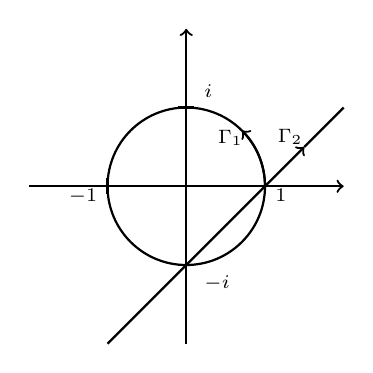
\begin{tikzpicture}
	% grid for draft only
	%%\draw [help lines] (-2,-2) grid (2,2);
	% the X-axis
	\draw[->,thick] (-2,0)--(2,0);
	\draw[thick] (-1,-0.1) -- (-1,0.1) node[below left] {\scriptsize $-1$};
	\draw[thick] (1,-0.1) -- (1,0.1) node[below right] {\scriptsize $1$};
	% the Y-axis
	\draw[->,thick] (0,-2)--(0,2);
	\draw[thick] (-0.1,-1) -- (0.1,-1) node[below right] {\scriptsize $-i$};
	\draw[thick] (-0.1,1) -- (0.1,1) node[above right] {\scriptsize $i$};
	% \Gamma_1
	\draw[thick] (0,0) circle (1);
	\draw[->,thick] (1,0) arc (0:45:1) node[below left=-4pt] {\scriptsize $\Gamma_1$};
	% \Gamma_2
	\draw[->,thick] (-1,-2) -- (1.5,0.5) node[above left=-3pt] {\scriptsize $\Gamma_2$};
	\draw[thick] (1.5,0.5) -- (2,1);
\end{tikzpicture}

